\chapter{Foundations}

In this chapter, we will discuss briefly the theory of gravitational wave -- how gravitational waves are manifested from the Einstein's equations. We will then delve deeper into GWs from the merger of two compact objects: we will discuss the mechanisms by which gravitational wave are generated and how to model these waves. Finally, we will discuss the potential mechanisms by which these binary mergers are formed and evolved, and how gravitational wave observations can provide insights into their origins. 

\subsubsection{\underline{Conventions}}
We define the conventions to describe the mathematical formalism of General Relativity. We will follow the convention of using latin indices to denote spatial vectors $i \in (x,y,z)$ and greek indices to denote space-time vectors $\mu \in (t, x, y, z)$ and follow the Einstein summation convention
\begin{align}
    a^{\mu}b_{\mu} = \sum_{\mu = 0}^{3} a^{\mu}b_{\mu}.
\end{align}

The \textit{metric tensor} $g_{\mu\nu}$ which defines the spacetime's local geometry is expressed as the line element $ds^2$ in a four-dimensional manifold \footnote{A manifold can be described as a collection of points, each of which, in a local vicinity, resembles the Euclidean space of dimension n, denoted as $\mathbb{R}^n$, where n represents the manifold's dimension.}
\begin{align}
    ds^2 = g_{\mu\nu}dx^{\mu}dx^{\nu}.
\end{align}
For flat space or \textit{Minkowski} metric, the convention is $\eta_{\mu\nu} = (-1, 1, 1, 1)$. We always use $c = G = 1$, unless stated otherwise. Partial differentials are simplified using $\partial_{\mu} = \dfrac{\partial}{\partial x^{\mu}}$.
The Cristoeffel symbol is given by:
\begin{align}
    \Gamma^{\rho}_{\mu\nu} = \dfrac{1}{2}g^{\rho\sigma}\big(\partial_{\mu}g_{\nu\sigma} + \partial_{\nu}g_{\mu\sigma} - \partial_{\sigma}g_{\mu\nu} \big).
\end{align}
The Riemann tensor is defined as:
\begin{align}
    R^{\mu}_{\nu\rho\sigma} = \partial_{\rho}\Gamma^{\mu}_{\nu\sigma} - \partial_{\sigma}\Gamma^{\mu}_{\nu\rho} + \Gamma^{\mu}_{\alpha\rho}\Gamma^{\alpha}_{\nu\sigma} - \Gamma_{\alpha\sigma}^{\mu}\Gamma^{\alpha}_{\nu\rho}.
\end{align}
The Ricci tensor is:
\begin{align}
    R_{\mu\nu} = R^{\alpha}_{\mu\alpha\nu},
\end{align}
and the Ricci scalar is 
\begin{align}
    R = g^{\mu\nu}R_{\mu\nu}.
\end{align}
The d'Alembertian operator is 
\begin{align}
    \Box = \partial^{\alpha}\partial_{\alpha} = -\dfrac{\partial^2}{\partial t^2} + \dfrac{\partial^2}{\partial x^2} + \dfrac{\partial^2}{\partial y^2} + \dfrac{\partial^2}{\partial z^2}.
\end{align}

\section{Gravitational wave theory}
Einstein's field equations form the cornerstone of General Relativity. They describe how matter and energy in the Universe shape space-time, and in turn, how this curved space-time dictates the motion of matter and energy. The equations are elegantly encapsulated in the formula:

\begin{align}
    R_{\mu \nu} - \dfrac{1}{2}g_{\mu \nu}R = 8\pi T_{\mu \nu},
    \label{Eq:Einstein_eq}
\end{align}
where $T_{\mu\nu}$ is the stress energy tensor describing the density and flux of energy and momentum. Some of the components of $T_{\mu\nu}$ could be understood as the following:
\begin{itemize}
    \item $T_{00}$ is the energy density.
    \item $T_{0i} = T_{i0}$ is the energy flux in the $i \in (x,y,z)$ direction or the density of $i$ momentum.
    \item $T_{ij}$ is the flux of $i$ momentum in the $j$ direction.
\end{itemize}
The rest of the quantities are described in the conventions.  

\subsection{Linearized gravity}
Solving Einstein's equation Eq. (\ref{Eq:Einstein_eq}) is complicated, and we simplify the metric tensor $g_{\mu\nu}$ by assuming small perturbations to the Minkowski tensor $\eta_{\mu\nu}$ by the gravitational field $h_{\mu\nu}$ such that
\begin{align}
    g_{\mu\nu} = \eta_{\mu\nu} + h_{\mu\nu},    \hspace{2cm}      \norm{h_{\mu\nu}} \ll 1.
\end{align}
We introduce a quantity called as \textit{trace reverse tensor} of $h_{\mu\nu}$ as
\begin{align}
    \bar{h}_{\mu\nu} = h_{\mu\nu} - \dfrac{1}{2}\eta_{\mu\nu}h,
\end{align}
where $h = \eta_{\mu\nu}h^{\mu\nu}$. The left side of the Einstein's equation can be simplified to the weak field limit in terms of $\bar{h}_{\mu\nu}$, as 
\begin{align}
    R_{\mu \nu} - \dfrac{1}{2}g_{\mu \nu}R = \dfrac{1}{2}\big( \partial^{\sigma}\partial_{\mu}\bar{h}_{\sigma\nu} -\partial^{\sigma}\partial_{\sigma}\bar{h}_{\mu\nu} + \partial_{\nu}\partial^{\alpha}\bar{h}_{\mu\alpha} - \eta_{\mu\nu}\partial^{\alpha}\partial^{\beta}\bar{h}_{\alpha\beta} \big),
\end{align}
where we keep only the terms linear in $h_{\mu\nu}$ and its derivatives, i.e. discarding any terms in of $\mathcal{O}(h^2)$.\\

The weak field Einstein's equations are invariant under small coordinate transformation to the metric such as translations
\begin{align}
    x'^{\mu} = x^{\mu} + \xi^{\mu}(x), \longrightarrow g'_{\mu\nu} = \eta_{\mu\nu} + h'_{\mu\nu},
\end{align}
and Lorentz rotations 
\begin{align}
    x'_{\mu} = \Lambda^{\mu}_{\nu}x^{\nu}, \longrightarrow g'_{\mu\nu} = \eta_{\mu\nu} + \Lambda_{\mu}^{\rho}\Lambda_{\nu}^{\sigma}h_{\rho\sigma}
\end{align}
where $\Lambda_{\mu}^{\rho}\Lambda_{\nu}^{\sigma}\eta_{\rho\sigma} = \eta_{\mu\nu}$. 

We can perform gauge transformations to use the \textit{Lorenz gauge}, such that
\begin{align}
    \partial^{\nu}\bar{h}_{\mu\nu} = 0,
\end{align}
and the linearized field equations are reduced to
\begin{align}
    \Box\bar{h}_{\mu\nu} = -16\pi T_{\mu\nu}.
\end{align}
Let us now consider vaccuum state solutions far away from any source of mass or energy, that is $T_{\mu\nu} = 0$, we obtain the travelling wave equation $\Box \bar{h}_{\mu\nu} = 0$. The solutions of which can be represented as a plan polarized travelling wave given by
\begin{align}
    \bar{h}_{\mu\nu} = A_{\mu\nu}e^{ik_{\alpha}x^{\alpha}},
\end{align}
where $A_{\mu\nu}$ is a complex matrix representing amplitude and phase of the plane waves, and $k^{\alpha} = (\omega, k^i)$ is the wave propagation vector satisfying the condition
\begin{align}
    k_{\alpha}k^{\alpha} = 0 = -\omega^2 + \norm{\vec{k}}^2.
\end{align}
This suggests that gravitational radiation propagates as plane waves, and since $\norm{\vec{k}} = \omega/v$, these waves must propagate at the speed of light ($v=1$). The Lorenz gauge is not unique, and we can apply a further gauge transformation that will satisfy the Lorenz gauge condition as long as the additional transformation satisfies the wave equation. Through these transformation, we obtain the relations
\begin{align}
    A_{\mu\nu}U^{\nu} = 0 \hspace{0.8cm} \text{and} \hspace{0.8cm} A^{\mu}_{ \mu} = 0,
\end{align}
where $U^{\nu}$ is a four-velocity. The first and second condition implies that gravitational waves are transverse and traceless respectively, and that $\bar{h}_{\mu\nu}^{TT} = h_{\mu\nu}^{TT}$. This gauge is known as the \textit{transverse-traceless gauge} (TT) which eliminates 8 out of 10 independent components of the symmetric perturbation tensor $h_{\mu\nu}$.

Considering a frame $e_{x}^{\mu}, e_y^{\nu}$ as the coordinate-basis unit vectors for the $x$ and $y-$coordinate respectively. The gravitational wave is assumed to be travelling along the $z-$direction. We define the two $+$ \textit{plus} and $\times$ \textit{cross} polarizations in terms of the basis as
\begin{align}
    e_{+}^{\mu\nu} &= e_x^{\mu}e_x^{\nu} - e_y^{\mu}e_y^{\nu},\\
    e_{\times}^{\mu\nu} &= e_x^{\mu}e_y^{\nu} + e_y^{\mu}e_x^{\nu}.
\end{align}
An arbitrary gravitational wave can then be expressed in terms of the superposition of these two polarizations in the TT gauge
\begin{align}
    h^{\mu\nu} = h_+(t,z)e^{\mu\nu}_{+} + h_{\times}(t,z)e_{\times}^{\mu\nu}.
\end{align}
and the perturbation metric tensor reads as 
\begin{align}
   h_{\mu\nu} =  \begin{bmatrix}
                0 & 0 & 0 & 0 \\
                0 & h_+ & h_{\times} & 0 \\
                0 & h_{\times} & -h_+ & 0 \\
                0 & 0 & 0 & 0 
                \end{bmatrix}
\end{align}
The two polarizations squeeze and stretch spaces between particles simultaneously and are rotated
$45^{\circ}$ relative to each other as shown in 
\begin{figure}
\centering
\begin{subfigure}{\textwidth}
  \centering
  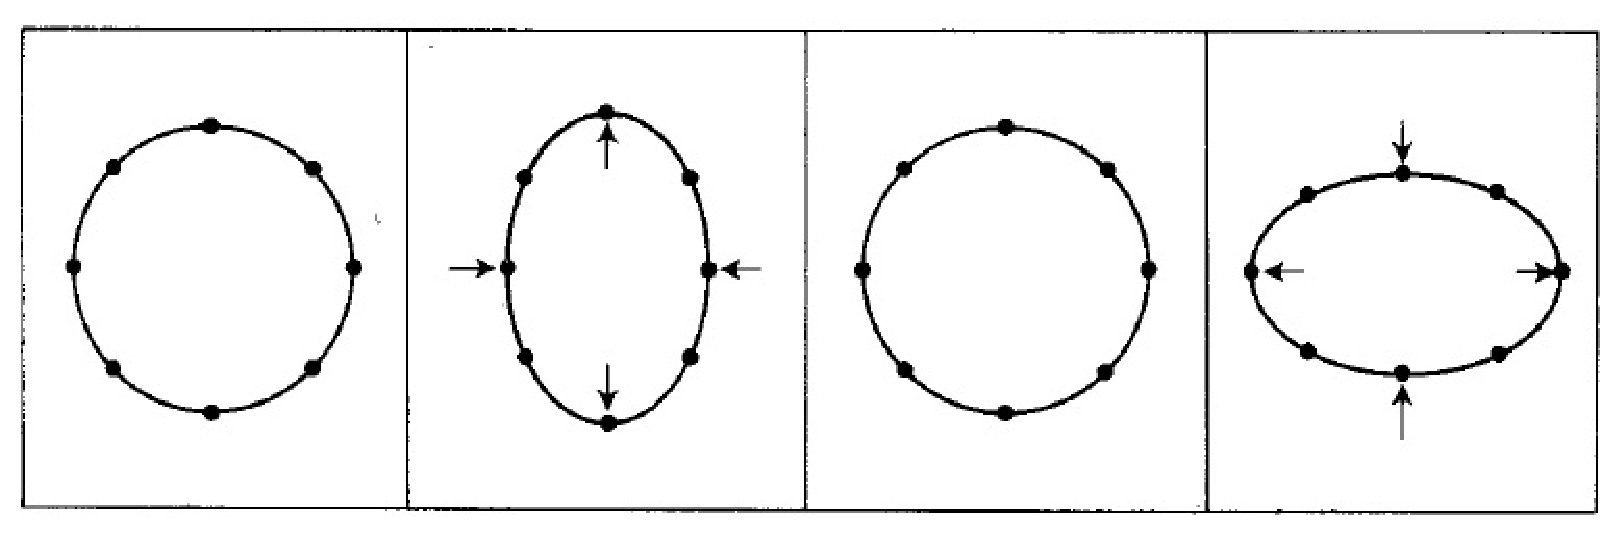
\includegraphics[width=0.5\linewidth]{figures/Introduction/pluspol.eps}
  \caption{effect of plus ($+$) polarisation}
  \label{fig:sub1}
\end{subfigure}\\
\begin{subfigure}{\textwidth}
  \centering
  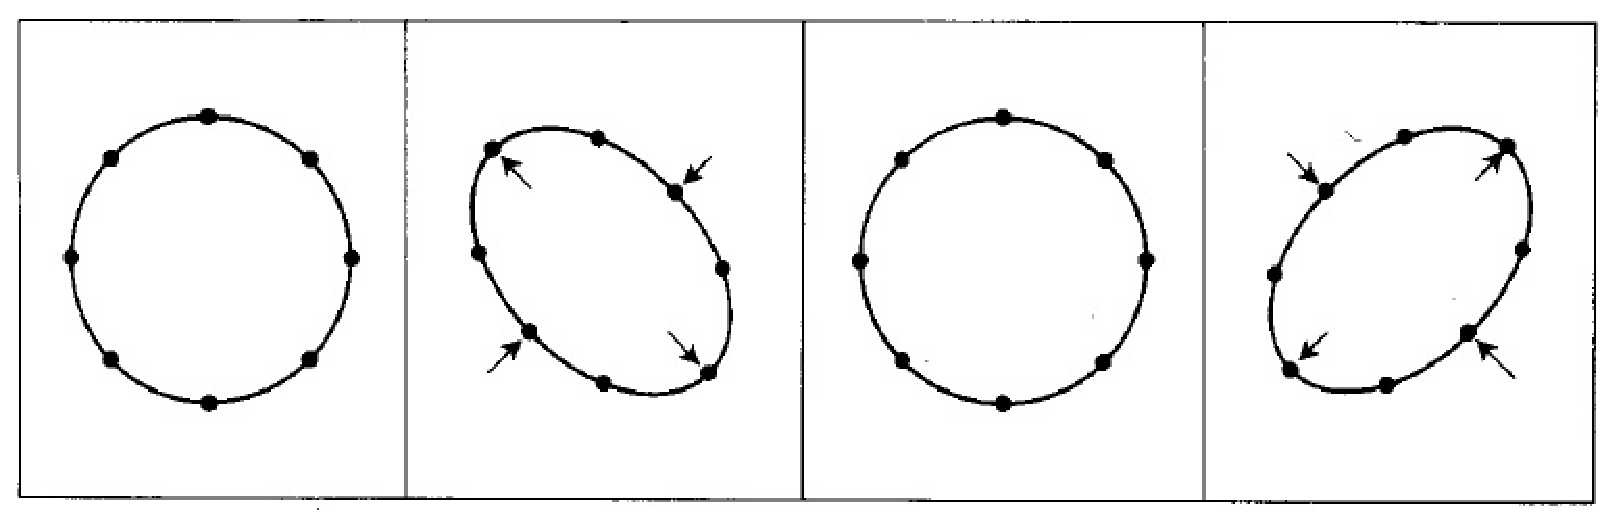
\includegraphics[width=0.5\linewidth]{figures/Introduction/crosspol.eps}
  \caption{effect of cross ($\times$) polarisation}
  \label{fig:sub2}
\end{subfigure}
\caption{Time sequence showing the effect of an oscillatory linear plane GW with (a) plus and (b) cross polarisation.}
\label{fig:Polarisation}
\end{figure}


\section{Compact Binary Mergers}

A binary system with compact objects such as black holes or neutron stars which are sufficiently close together will emit energy via the gravitational radiation. As the system evolves in frequency the radiated energy increases and the compact objects in-spiral each other. 
These are currently the most commonly detected sources of gravitational waves. 

\subsection{Modeling compact binary mergers}

A compact binary merger involves two massive objects in a close orbit, spiraling inwards due to the emission of gravitational waves, until they eventually merge. The signal from such an event can be characterized by various parameters, including the masses and spins of the two objects, the distance to the source, the inclination of the orbital plane relative to the observer, and the sky location of the source.


Different Binaries and Mathematical Formalisms:
Binary Black Holes (BBH): BBH mergers involve two black holes spiraling inwards and merging. The post-Newtonian formalism, which provides a series expansion in terms of the velocity of the objects divided by the speed of light, can be used to describe the inspiral phase. For the merger and ringdown phases, numerical relativity simulations are required, as the gravitational fields are extremely strong and the dynamics are highly nonlinear.

Binary Neutron Stars (BNS): BNS mergers involve two neutron stars. In addition to the gravitational wave emission, these events can also result in electromagnetic signals, such as gamma-ray bursts. The inspiral can be modeled using post-Newtonian formalism, but tidal effects (which are important for neutron stars) must also be taken into account. Numerical relativity simulations are required to accurately model the merger and post-merger phases, including the potential formation of a hypermassive neutron star or a black hole.

Neutron Star – Black Hole Binaries (NSBH): These binaries involve a neutron star and a black hole. The modeling of these systems is similar to BNS mergers, but with additional complexity due to the interaction of the neutron star with the black hole’s tidal field, which can lead to the disruption of the neutron star.

\subsection{Orbital mechanics and the Post Newtonian treatment}

Gravitational waves are generated by the change in the quadrupolar moment which can occur for sources that are broadly classified in four different types. \\

\begin{itemize}
\item Continuous Gravitational Waves
\item Stochastic Gravitational Wave Background
\item Supernovae
\item Primordial Gravitational Waves
\end{itemize}


\subsection{Gravitational waveforms}

Gravitational waves can be modeled by numerically solving the Einstein equations. 

A gravitational wave signal from a compact binary merger can be divided into three main parts:
Inspiral: The phase where the two objects are orbiting each other, gradually coming closer. The waveform in this phase can be approximated using post-Newtonian theory or effective-one-body formalism.

Merger: The phase where the two objects coalesce. PN approximations begin breaking down as these objects come closer. Analytical approximations are no longer valid and thus, this phase requires numerical relativity simulations for accurate modeling.

Ringdown: The phase after the merger, where the newly formed object (a black hole or a neutron star) settles into its final state, emitting gravitational waves in the process. The ringdown can be modeled using black hole perturbation theory, specifically quasi-normal modes.

Various waveform models have been proposed and developed to describe the full signal from compact binary mergers, combining analytical and numerical techniques. These include:

Phenomenological Models: These models use analytical fits to numerical relativity simulations to describe the entire waveform. Phenomenological models for gravitational waves from coalescing binary systems (such as binary black holes or neutron stars) are crucial for the detection and interpretation of gravitational wave signals. These models aim to provide accurate and computationally efficient descriptions of the signals across all phases of the coalescence: inspiral, merger, and ringdown. Below, I will delineate the construction of phenomenological waveform models, highlighting the key steps and methodologies involved.

1. Inspiraling Phase: Post-Newtonian Theory
    Post-Newtonian Expansion: The inspiral phase, where the binary components are far apart and moving slowly compared to the speed of light, is modeled using post-Newtonian (PN) theory. This involves expanding the equations of motion and gravitational waveforms in powers of $v/c$ (velocity of the bodies divided by the speed of light).

    Incorporating Spin Effects: The effects of the spins of the binary components are included using spin-orbit and spin-spin coupling terms in the post-Newtonian expansion.

    Higher-Order Corrections: The accuracy of the model is improved by including higher-order PN terms. The coefficients of these terms are calculated analytically or fitted to numerical relativity simulations.

2. Merger Phase: Numerical Relativity
    Numerical Simulations: The merger phase, where the binary components are in close proximity and moving at a significant fraction of the speed of light, requires numerical relativity simulations to accurately model. These simulations involve solving Einstein’s equations directly on a computer grid.

    Fitting to Numerical Data: The parameters of the phenomenological model are tuned to provide the best match to the numerical relativity waveforms. This process may involve fitting formulae that describe how the waveform changes with different binary parameters (such as masses and spins).

3. Ringdown Phase: Black Hole Perturbation Theory
    Quasi-Normal Modes: After the merger, the resulting single black hole undergoes a ringdown phase, emitting gravitational waves as it settles to a stable state. This phase is modeled using black hole perturbation theory, identifying the quasi-normal modes of the final black hole.

    Matching to Merger: The ringdown waveform is matched onto the end of the merger waveform, ensuring a smooth transition between the two phases.

Creating a Complete Model
    Matching Across Phases: The inspiral, merger, and ringdown phases are combined to create a complete waveform model. This requires careful matching of the waveforms at the boundaries between the phases to ensure consistency and accuracy.

    Parameterization: The complete model is parameterized in terms of the physical parameters of the binary system, such as the component masses, spins, and orbital parameters. This allows for rapid generation of waveforms for different binary configurations.

5. Validation and Calibration
    Comparison to Numerical Relativity: The phenomenological model is validated by comparing its predictions to a wide range of numerical relativity waveforms, ensuring accuracy across the parameter space.

    Calibration: The model may be calibrated to improve agreement with numerical relativity simulations, particularly in regions of the parameter space where the post-Newtonian or perturbative approximations are less accurate.

6. Application in Data Analysis
    Rapid Waveform Generation: The phenomenological model allows for the rapid generation of waveforms, which is essential for gravitational wave data analysis, including signal detection and parameter estimation.
    
    Coverage of Parameter Space: The model is designed to accurately cover the entire parameter space of binary coalescences, allowing for the analysis of a wide range of binary systems.


Effective-One-Body (EOB) Models: These models map the two-body problem onto an effective one-body problem, using results from post-Newtonian theory and numerical relativity. It was initially developed to overcome the limitations of post-Newtonian theory in the highly relativistic regime of binary mergers. 

1. Conceptual Foundation

The EOB method transforms the problem of two interacting bodies in a binary system into an equivalent problem of a single test particle moving in an effective external gravitational field. This effective field encapsulates the complex interactions between the two bodies. The transformation simplifies the problem, making it more tractable, especially in the strong-field, fast-motion regime close to merger.

2. Mapping to an Effective Problem
    Effective Metric: An effective metric is introduced to describe the gravitational field in which the test particle moves. This metric is parameterized in terms of the masses and spins of the binary components.

    Reduced Mass and Total Mass: The dynamics are described in terms of the reduced mass $\mu=\dfrac{m_1m_2}{m_1+m_2}$ and the total mass $M=m_1+m_2$, where $m_1$ and $m_2$ are the masses of the two bodies.

    Hamiltonian: An effective Hamiltonian is constructed to describe the motion of the test particle. This Hamiltonian includes not only the leading-order (Newtonian) terms but also higher-order post-Newtonian corrections and resummed terms that capture strong-field effects.

3. Resumming Post-Newtonian Terms
    Padé Approximants: The post-Newtonian series is resummed using techniques like Padé approximants to improve its convergence and extend its validity into the strong-field regime.

    Resummation of the Energy Flux: The energy flux of gravitational waves emitted by the system is also resummed to improve its behavior in the strong-field, fast-motion regime.

4. Calibration to Numerical Relativity
    Tuning Free Parameters: The EOB model includes several free parameters that cannot be determined purely analytically. These parameters are calibrated by comparing EOB predictions to fully numerical solutions of Einstein’s equations for binary systems, obtained via numerical relativity simulations.

    Improving the Model: The calibration process helps in refining the EOB model, ensuring that it accurately captures the complex dynamics of binary coalescence, especially during the merger and ringdown phases.

5. Waveform Generation
    Generating Inspirals: The EOB approach generates waveforms for the inspiral phase of the binary coalescence, capturing the increasing amplitude and frequency of the gravitational waves as the bodies spiral together.

    Extending to Merger and Ringdown: By incorporating information from numerical relativity, the EOB model is extended to accurately describe the merger of the two bodies and the ringdown of the resulting single compact object.

6. Application in Gravitational Wave Astronomy
    Parameter Estimation: EOB models are crucial for interpreting gravitational-wave signals detected by observatories like LIGO and Virgo, allowing for the extraction of physical parameters of the binary system.

    Real-time Data Analysis: Due to their efficiency in generating waveforms, EOB models are particularly useful for real-time data analysis and rapid characterization of gravitational-wave events.

7. Continuous Development and Validation
    Incorporating Spin and Precession: Efforts are ongoing to improve EOB models by incorporating effects like spin-precession and higher-order mode contributions, which are important for accurately modeling systems with spinning and misaligned components.

    Validation Across the Parameter Space: EOB models are continuously validated and updated based on comparisons with new numerical relativity simulations, ensuring their reliability across the vast parameter space of binary configurations.


Hybrid Models: These models combine post-Newtonian or EOB waveforms for the inspiral with NR waveforms for the merger and ringdown.


\section{Formation and evolution mechanisms of binary mergers}

Neutron stars (NS) and black holes (BH) with stellar masses typically emerge from the end stages of massive stars. These massive stars are usually not solitary; they often exist in pairs or even more complex groups, with many engaging in interactions with their companions, as illustrated in the works of Sana et al. (2012) and Moe and Di Stefano (2017). The dynamics of these interactions, which significantly shape the destiny and observable traits of the stars—as well as the events they catalyze, like double compact object (DCO) mergers—are not fully understood .

Gravitational wave (GW) detections offer a promising avenue for unveiling the intricate mechanisms governing the life cycles of these massive stellar entities. Yet, when such NS or BH formations are situated in regions bustling with stellar activity, the frequent stellar run-ins can modify their characteristics significantly. Under these circumstances, repeated mergers are a possibility, hinting that some GW events we observe may involve BHs that are not straightforwardly linked to the immediate outcomes of stellar or binary evolution.

One of the primary complexities in the field of GW astrophysics is the ambiguity in interpreting observational data, which can vary based on the postulated history of the merger's formation . Therefore, distinguishing the unique origins of merger events based on their observational signatures is of paramount importance.

An illustrative example is provided by the most massive GW event on record to date (GW190521), which was interpreted as a merger between two BHs with a combined mass of 150 $M_{\odot}$, with the primary BH weighing over 65 $M_{\odot}$ at a 99\% confidence level (refer to Abbott et al. 2020b,c, and see also Fishbach and Holz 2020 for a perspective that a mass over 120 $M_{\odot}$ is plausible). The formation of such a massive BH through isolated binary evolution is deemed highly improbable, as it would typically be in the range of 50 $M_{\odot}$ to 120 $M_{\odot}$ — a region expected to yield no remnant due to pair-instability supernovae (PISN), according to predictions by Bond et al. (1984) and Woosley and Heger (2006). Should GW190521 indeed include a BH mass within this predicted gap, it would strongly suggest an origin outside of isolated binary star evolution.

However, drawing broader conclusions about the evolution of massive stars from singular observations requires an understanding of how typical such instances are. As the pool of GW data grows, it allows for a more detailed understanding of the properties of local DCO mergers, such as the rates at which they occur and their mass distributions. Weaker constraints exist on their spin distributions and sky localizations, which could indicate potential host galaxies.

One particularly interesting discovery is that the bulk of the BHBH mergers observed—32 out of 44 systems—feature at least one BH exceeding 30 $M_{\odot}$ in mass. The prevalence of such massive BHs among GW findings, while anticipated due to selection biases (discussed in Sec. 1.1.2), is noteworthy since electromagnetically observed systems with BHs before the era of GW detection were estimated to be less than 20 $M_{\odot}$ (e.g., Tetarenko et al., 2016; Miller-Jones et al., 2021). The maximum mass achievable by a BH from stellar origin is understood to be metallicity-dependent, with wind mass loss rates during the massive star phase increasing with metal content, thus reducing the final mass of the BH (Vink et al. 2001; Vink and de Koter 2005). This has led to theories that the massive BHBH mergers detected through GWs may arise from low-metallicity star formation regions or potentially from previous merger events.

The potential for gravitational wave data to reveal discontinuities, such as mass gaps or cutoffs, within the compact object mass spectrum is of significant interest for its implications on core collapse and stellar explosion physics. Differing explosion models predict varying outcomes, such as a mass gap between approximately 3 - 5 $M_{\odot}$ due to the dynamics of massive stellar core collapse, with others anticipating a more uniform distribution (for instance, see Fryer et al., 2012). GW data can thus provide valuable constraints on these theoretical models.

The advancement in detector sensitivity is starting to allow examination of the BHBH population across cosmic time. The anticipated evolution of GW detector capabilities, with projects like Cosmic Explorer and Einstein Telescope (outlined by Reitze et al. 2019 and Maggiore et al. 2020), promises to map this dependency across the span of cosmic star formation history. Such insights could enhance our comprehension of the Universe's chemical evolution and its correlation with unresolved questions. This chapter will provide a comprehensive overview of these formation and evolution mechanisms.

\textbf{Formation channels}

\textbullet{Primordial Formation}

Some compact binaries are believed to form directly from the primordial gas in the early Universe. These binaries originate from density fluctuations in the early Universe, leading to the formation of closely-packed binaries.

\textbullet{Tidal Capture}

In dense stellar environments like globular clusters, stars can come close enough for tidal forces to dissipate energy and form a bound pair. Over time, through dynamical interactions and gravitational radiation, these pairs can evolve into compact binaries.

\textbf{Evolutionary Pathways}

\textbullet{Common Envelope Phase}

One of the most significant phases in the evolution of compact binary systems is the common envelope (CE) phase. This occurs when one of the stars in the binary expands, engulfing its companion. Drag forces within the envelope can cause the companion to spiral inward, leading to a closer binary system. If enough energy is released, the envelope can be ejected, leaving behind a compact binary.

\textbullet{Mass Transfer}

After the CE phase or in the absence of it, one star can transfer mass to its companion. Depending on the mass ratio and other properties, this mass transfer can be stable or unstable, leading to different outcomes:

    Roche Lobe Overflow (RLOF): When a star fills its Roche lobe, the outer layers can be transferred to its companion. This process can lead to drastic changes in the binary configuration.

    Thermal Timescale Mass Transfer: In cases where the mass-losing star is much more massive than its companion, the mass transfer can be rapid, leading to the formation of a helium core.

\textbullet{Stellar Collisions}

In dense stellar environments, direct collisions between stars can lead to the formation of compact binaries. These collisions can merge two stars or strip the outer layers of one, leaving behind a compact remnant.

\textbullet{Gravitational Radiation}

Compact binaries, especially those involving neutron stars or black holes, can emit gravitational waves. This radiation causes the binary to lose energy, leading to a decrease in the orbital separation and eventually merger.

\textbf{End Stages}

\textbullet{Supernova Explosions}

If one component of the binary undergoes a supernova explosion, it can disrupt the binary. Alternatively, if the binary remains bound, the system may evolve into a compact binary with a neutron star or a black hole.

\textbullet{Mergers}

When the separation between binary components decreases to a critical value, the binary can merge, leading to various outcomes:

    White Dwarf Mergers: Can lead to a type Ia supernova.

    Neutron Star Mergers: Result in the emission of intense gravitational waves and can form a black hole.

    Black Hole Mergers: Produce powerful gravitational waves detectable by observatories like LIGO and Virgo.





